\documentclass[12pt]{cours}

\title{\textbf{\textsc{Diagramme des classes}}}
\author{Delay Emmanuel -- Desforêts Nicolas}


\usepackage{pgf-umlcd}



\begin{document}

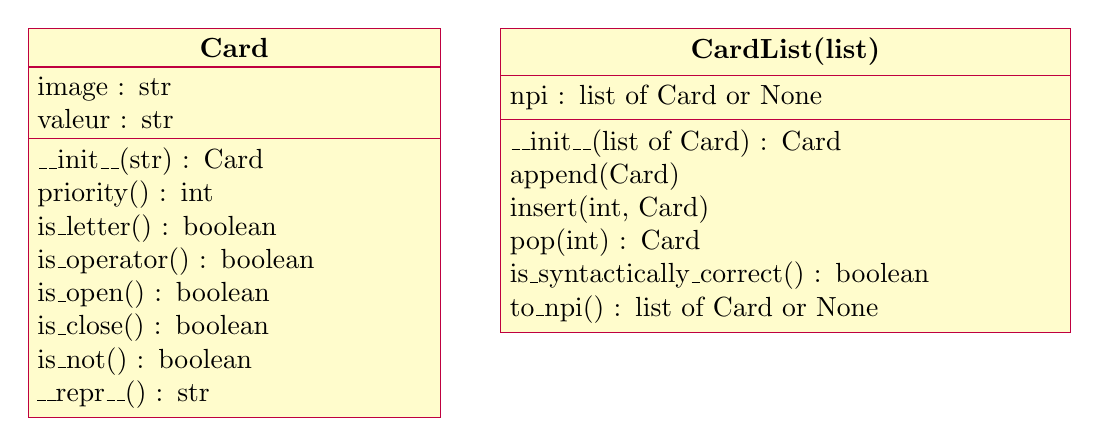
\begin{tikzpicture}
\begin{class}{Card}{0, 0}
\attribute{image : str}
\attribute{valeur : str}
\operation{\_\_init\_\_(str) : Card}
\operation{priority() : int}
\operation{is\_letter() : boolean}
\operation{is\_operator() : boolean}
\operation{is\_open() : boolean}
\operation{is\_close() : boolean}
\operation{is\_not() : boolean}
\operation{\_\_repr\_\_() : str}
\end{class}
\begin{class}[text width=7cm]{CardList(list)}{7,0}
\attribute{npi : list of Card or None}
\operation{\_\_init\_\_(list of Card) : Card}
\operation{append(Card)}
\operation{insert(int, Card)}
\operation{pop(int) : Card}
\operation{is\_syntactically\_correct() : boolean}
\operation{to\_npi() : list of Card or None}
\end{class}
\end{tikzpicture}


\end{document}

